%\documentclass[12pt]{article}
\documentclass[12pt,titlepage,oneside,final]{book}


\usepackage[a4paper,top=3cm,bottom=3cm,right=3cm, left=4cm]{geometry}
\usepackage{times}
\usepackage{subcaption}
\usepackage{lipsum}
\usepackage{graphicx}
\usepackage{sectsty}
\usepackage[T1]{fontenc}

\usepackage{enumitem}
\usepackage{array}
\usepackage{booktabs}
\usepackage{multirow}
\usepackage{multicol}

%%%%%%%%%%%%%%%%%%%%%%%%%%%%%
%                           %
%     hyperlink setting     %
%                           %
%%%%%%%%%%%%%%%%%%%%%%%%%%%%%
\usepackage{hyperref}       %
\hypersetup{                %
    colorlinks,             %
    citecolor=black,        %
    filecolor=black,        %
    linkcolor=black,        % 
    urlcolor=black          %
}                           %
%%%%%%%%%%%%%%%%%%%%%%%%%%%%%



%%%%%%%%%%%%%%%%%%%%%%%%%%%%%%%%%%%%%%%%%%%%%%%%%
%      Rename cot, list figure, list table      %
%%%%%%%%%%%%%%%%%%%%%%%%%%%%%%%%%%%%%%%%%%%%%%%%%

%\renewcommand{\abstractname }{ABSTRAK}
\renewcommand{\contentsname }{DAFTAR ISI}
\renewcommand{\listfigurename }{DAFTAR GAMBAR}
\renewcommand{\listtablename }{DAFTAR TABEL}
%\renewcommand{\bibname}{DAFTAR PUSTAKA}

%\renewcommand{\refname}{DAFTAR PUSTAKA}

%%%%%%%%%%%%%%%%%%%%%%%%%%%%%%%%%%%%%%%%%%%%%%%%%

\allsectionsfont{\normalsize\bfseries}

%\input{hangilastyle}
%\addbibresource{daftar-pustaka.bib}
%%%%%%%%%%%%%%%%%%%%%%%%%%%%%%%%%%%%%%%%%%%%%%%%%%%%%%%%%%%%%%%%%%%%%%%%%%%
%                          Rename figure, table                           %
%%%%%%%%%%%%%%%%%%%%%%%%%%%%%%%%%%%%%%%%%%%%%%%%%%%%%%%%%%%%%%%%%%%%%%%%%%%

\captionsetup[figure]{labelfont={it},name={Gambar},labelsep=period}
\captionsetup[table]{labelfont={it},name={Tabel},labelsep=period}

%%%%%%%%%%%%%%%%%%%%%%%%%%%%%%%%%%%%%%%%%%%%%%%%%%%%%%%%%%%%%%%%%%%%%%%%%%%

%\usepackage{float}
%\floatstyle{plaintop}
%\restylefloat{table}
%\usepackage[tableposition=top]{caption}

\usepackage{chngcntr}
\counterwithin{figure}{section}
\counterwithin{table}{section}


\usepackage{amsmath}  
\numberwithin{equation}{section}

\usepackage{caption}
\numberwithin{figure}{section}

\newcommand*{\appheading}[1][Appendix]{%
  \setcounter{secnumdepth}{0}\section{#1}\setcounter{secnumdepth}{3}%
  \renewcommand*{\thesubsection}{\Alph{subsection}}
  \numberwithin{equation}{subsection}
  \numberwithin{figure}{subsection}
}


\usepackage[utf8]{inputenc}
\usepackage{graphicx}
\graphicspath{ {images/} }

\setcounter{tocdepth}{3}
\setcounter{secnumdepth}{3}
\usepackage{lipsum}

\newcommand{\chaptertitleformat}{%
  \thechapter.\ \chaptername\space \Roman{chapter}%
}



% \usepackage{sectsty}
% \allsectionsfont{\centering}

\title{Laporan Magang}
\author{Prisilia Ines}

% \date{}

\usepackage{blindtext}
\usepackage[pagestyles]{titlesec}
\newpagestyle{main}{\setfoot{}{}{\thepage}}
\pagestyle{main}
\assignpagestyle{\chapter}{main}

\usepackage{fancyhdr,lipsum}

\fancypagestyle{frontmatter}{%
  \pagestyle{plain}% Just like plain page style
  \fancyfoot[C]{\roman{page}}% Roman page number in footer centre
}


\let\oldfrontmatter\frontmatter
\renewcommand{\frontmatter}{
  \oldfrontmatter
  \pagestyle{frontmatter}
}
\let\oldmainmatter\mainmatter
\renewcommand{\mainmatter}{
  \oldmainmatter
  \pagestyle{mainmatter}
}

\usepackage{titlesec}
\titleformat{\section}[block]{\normalsize\bfseries\filcenter}{}{1em}{}
\titleformat{\chapter}[block]{\normalsize\bfseries\filcenter}{}{1em}{}

\usepackage[utf8]{inputenc}

\setlength{\parindent}{4em}
\setlength{\parskip}{1em}
\renewcommand{\baselinestretch}{1.5}

\usepackage{indentfirst}



\usepackage{etoolbox,refcount}
\usepackage{multicol}

\newcounter{countitems}
\newcounter{nextitemizecount}
\newcommand{\setupcountitems}{%
  \stepcounter{nextitemizecount}%
  \setcounter{countitems}{0}%
  \preto\item{\stepcounter{countitems}}%
}
\makeatletter
\newcommand{\computecountitems}{%
  \edef\@currentlabel{\number\c@countitems}%
  \label{countitems@\number\numexpr\value{nextitemizecount}-1\relax}%
}
\newcommand{\nextitemizecount}{%
  \getrefnumber{countitems@\number\c@nextitemizecount}%
}
\newcommand{\previtemizecount}{%
  \getrefnumber{countitems@\number\numexpr\value{nextitemizecount}-1\relax}%
}
\makeatother    
\newenvironment{AutoMultiColItemize}{%
\ifnumcomp{\nextitemizecount}{>}{3}{\begin{multicols}{2}}{}%
\setupcountitems\begin{itemize}}%
{\end{itemize}%
\unskip\computecountitems\ifnumcomp{\previtemizecount}{>}{3}{\end{multicols}}{}}


\usepackage{fancyhdr}
  \fancyhf{}
  \renewcommand{\headrulewidth}{0pt}
  \fancyhf[cf]{\thepage}
  \pagestyle{fancy}

%%%%%%%%%%%%%%%%%%%%%%%%%%%%%
%                           %
%%%%%%%%%%%%%%%%%%%%%%%%%%%%%

\begin{document}

\pagenumbering{roman}


\mychap{1}{HALAMAN PERSETUJUAN}{HALAMAN PERSETUJUAN}

\begin{center}
    
\textbf{Laporan Kerja Magang dengan judul\linebreak[1]}

\textbf{ IMPLEMENTASI FRAMEWORK HUGO \\
    PADA WEBSITE PROFIL PERUSAHAAN \\
    (STUDI KASUS: PT. BOGA PANGAN SENTOSA)}
\end{center}


\begin{center}
oleh\\
Prisilia Ines\\
00000018075\linebreak[2]

\textbf{telah disetujui untuk diajukan pada \\ 
        Sidang Kerja Magang Universitas Multimedia Nusantara\linebreak[2]}
\end{center}

\begin{center}

    \begin{tabular}{p{0cm}c}
        &Tangerang, 26 September 2019\\
        &Menyetujui\\
        &Dosen Pembimbing\\
        &\\
        &\\
        &{Adhi Kusnadi, S.T., M.Si.}
    \end{tabular}

    \begin{tabular}{p{0cm}c}
        &Mengetahui,\\
        &Ketua Program Studi\\
        &\\
        &\\
        &{Seng Hansun S.Si., M. Cs.}
    \end{tabular}
    
\end{center}


\clearpage
\mychap{1}{Lembar Pernyataan}{Lembar Pernyataan tidak melakukan plagiat \\ dalam penyusunan Laporan Kerja Magang}

\noindent Dengan ini saya:
\begin{flushleft}
    \begin{tabular}{ll}
    Nama          & : Prisilia Ines \\
    Nama          & : Prisilia Ines \\
    NIM           & : 00000018075   \\
    Program Studi & : Informatika  
    \end{tabular}
\end{flushleft}
\noindent Menyatakan bahwa saya telah melaksanakan praktek kerja magang:
\begin{flushleft}    
    \begin{tabular}{ll}
    Nama perusahaan & : PT. Boga Pangan Sentosa          \\
    Divisi          & : ICT                              \\
    Alamat          & : Perumnas Teluk Jambe, Karawang   \\
    Periode Magang  & : 17 Juni 2019 – 18 September 2019
    \end{tabular}
\end{flushleft}
    \noindent Laporan kerja magang merupakan hasil karya saya sendiri, dan saya tidak melakukan plagiat. 
    Semua kutipan karya ilmiah orang lain atau lembaga lain yang dirujuk dalam laporan 
    kerja magang ini telah saya sebutkan sumber kutipannya serta saya cantumkan di Daftar Pustaka
Jika kemudia hari terbukti ditemukan kecurangan/ penyimpangan, baik dalam pelaksanaan kerja 
magang maupun dalam penulisan laporan kerja magang, saya bersedia menerima konsekuensi dinyatakan 
tidak lulus untuk mata kuliah kerja magang yang telah saya tempuh.\\

\noindent \begin{tabular}{l}
Tangerang, 9 September 2019 \\
                            \\
                            \\
                            \\
Prisilia Ines              
\end{tabular}

\clearpage
\mychap{1}{ABSTRAKSI}{IMPLEMENTASI FRAMEWORK HUGO \\
        PADA WEBSITE PROFIL PERUSAHAAN \\
     (STUDI KASUS: PT. BOGA PANGAN SENTOSA)}

Perkembangan teknologi terutama \emph{internet} dan sistem online akhir-akhir ini sangat pesat 
yang menyebabkan persaingan usaha semakin ketat. Hampir semua orang yang mempunyai komputer 
dan \emph{smart-phone} yang terkoneksi dengan \emph{internet}, oleh karena itu \emph{website} perusahaan harus berisi 
profil perusahaan dan jasa atau produk yang disediakan menjadi langkah awal agar memenangkan persaingan. 
\emph{website} memiliki peran penting dalam suatu bisnis seperti meningkatkan pengetahuan dan kepercayaan pembeli 
terhadap perusahaan. PT. Boga Pangan Sentosa (PT. BPS) merupakan perusahaan yang bergerak di bidang katering 
makanan untuk perusahaan industri. Namun, PT. BPS masih belum menerapkan strategi \emph{branding} yang efektif. 
Dengan adanya \emph{website} profil perusahaan, dapat meningkatkan reputasi dari perusahaan agar menjadi daya tarik 
pembeli dan membangun jaminan kualitas. \emph{website} profil perusahaan akan dikembangan dengan \emph{framework} Hugo. 
Hugo adalah situs \emph{statis generator} yang ditulis dengan bahasa Go. Hugo memiliki performa kecepatan \emph{website} 
dalam menyajikan konten, kemudahan dalam memperbaiki dan memperbaharui \emph{website} dikemudian hari, tampilan yang 
minimalis, serta \emph{website} dapat ditemukan dengan mudah pada \emph{search engine}.  Situs \emph{statis generator} 
fokus pada 
pekerjaan utama yaitu menghasilkan situs berbasis HTML yang tidak bergantung pada \emph{database} atau sumber data 
eksternal lainnya karena menghindari pemrosesan sisi server saat mengakses \emph{website}. 
Diharapkan dengan tersedianya \emph{website} PT. BPS ini diharapkan dapat meningkatkan kehadirannya, 
karena calon pelanggan dapat melihat informasi perusahaan secara detail kapan saja (365d x 24h). 
Oleh karena itu, \emph{website} yang dibuat harus berisi informasi lengkap dan menarik pelanggan serta dapat 
dengan kecepatan yang tinggi. 

\noindent Kata Kunci: \emph{Framework} Hugo, Go Lang, Situs \emph{Statis Generator}, \emph{website} Profil Perusahaan.

\clearpage
\begin{center}
    \textbf{Kata Pengantar}
    \addcontentsline{toc}{section}{Kata Pengantar}
\end{center}

%\setcounter{section}{3}
%\setcounter{subsection}{0}

Puji syukur kepada Tuhan Yang Maha Esa, atas terselesaikannya kerja magang di PT. Boga Pangan Sentosa. 
Laporan Magang ini dibuat untuk memenuhi persyaratan tugas mata kuliah kerja magang di bidang Informatika. 
%Tujuan dibuatnya laporan magang ini kaitannya dengan dunia kerja di PT. Boga Pangan Sentosa. 
Dalam penyusu-\newline nan laporan magang tidak terlepas dari bimbingan dari berbagai pihak. 
Maka penulis ucapkan rasa hormat dan terimakasih kepada semua pihak yang telah 
memberikan dukungan sampai selesainya laporan magang ini.
Penulis juga mengucapkan terima kasih kepada:
\begin{enumerate}
    \item Bapak Dr. Ninok Leksono, Rektor Universitas Multimedia Nusantara yang memberi inspirasi bagi penulis untuk berprestasi,
    \item Ibu Friska Natalia, Ph.D., Dekan Fakultas Tenik dan Informatika Universitas Multimedia Nusantara,
    \item Bapak Seng Hansun S.Si., M. Cs. , Ketua Program Studi Informatika Universitas Multimedia Nusantara, yang menerima penulis dengan baik untuk berkonsultasi dan
    \item Bapak. Adhi Kusnadi, S.T., M.Si yang membimbing pembuatan laporan Kerja Magang dan yang telah mengajar penulis tata cata menulis karya ilmiah dengan benar.
\end{enumerate}
    Penulis juga mengucapkan terima kasih kepada keluarga dan teman-teman yang memberikan dukungan doa dan semangat pada penulis.
Semoga laporan Kerja Magang ini dapat bermanfaat, baik sebagai sumber informasi maupun sumber inspirasi, bagi para pembaca.

\begin{tabular}{p{7.5cm}r}
&Tangerang, September 2019\\
&\\
&\\
&\\
&{Prisilia Ines}
\end{tabular}


\tableofcontents
\listoffigures
\clearpage
\listoftables
%\usepackage{tabularx}

\clearpage
\pagenumbering{arabic}
%\section[BAB I PENDAHULUAN]{BAB I\\ PENDAHULUAN}

%\addtocounter{subsection}{1}

\begin{center}
    \textbf{BAB I \\ PENDAHULUAN}
    \addcontentsline{toc}{chaper}{BAB I PENDAHULUAN}
\end{center}

\setcounter{section}{1}
\setcounter{subsection}{0}

\subsection{Latar Belakang}

Perkembangan teknologi terutama \emph{internet} dan sistem \emph{online} akhir-akhir ini sangat pesat 
yang menyebabkan persaingan usaha semakin ketat. Pengusaha harus mempunyai suatu strategi yang inovatif, 
yaitu menerapkan teknologi informasi untuk memenangkan persaingan agar menjadi pemimpin pasar \emph{(market leader)}.

Langkah awal dalam penerapan teknologi ini adalah dengan membuat sebuah \emph{website} perusahaan, 
karena masyarakat sudah terbiasa untuk mencari informasi seperti produk dan jasa melalui \emph{internet}. 
Hampir semua orang yang mempunyai komputer dan \emph{smart-phone} yang terkoneksi dengan \emph{internet}, oleh karena itu 
\emph{website} perusahaan berisi profil perusahaan dan jasa / produk yang disediakan 
menjadi langkah awal agar memenangkan persaingan.

Salah satu langkah yang dapat dilakukan untuk dapat bersaing dalam dunia bisnis yaitu dengan membuat suatu \emph{website} perusahaan. 
\emph{website} memiliki peran penting dalam suatu bisnis 
seperti meningkatkan pengetahuan dan kepercayaan pembeli terhadap perusahaan. 
Dengan kata lain, \emph{website} banyak dilakukan untuk meningkatkan \emph{brand} image perusahaan. 
Informasi dapat diakses dimana saja dan kapan saja  selama ada koneksi \emph{internet}. 
Biaya pemasaran lebih murah dibandingkan dengan cara tradisional yang dahulu mencetak brosur dan sebagainya.

PT. Boga Pangan Sentosa (PT. BPS) merupakan perusahaan yang bergerak di bidang katering makanan untuk perusahaan industri. 
Namun, PT. BPS masih belum menerapkan strategi branding yang efektif karena sampai saat ini dilakukan dengan cara kuno. 
Branding bertujuan untuk membangun citra dari perusahaan. Dengan adanya \emph{website} profil perusahaan, 
dapat meningkatkan reputasi dari perusahaan agar menjadi daya tarik pembeli dan membangun jaminan kualitas.

Dalam pembuatan \emph{website}, diperlukan penelitian untuk menentukan \emph{Content Management System} (CMS) 
yang tepat dan sesuai dengan kriteria. Hal yang menjadi perbandingan seperti performa kecepatan \emph{website} 
dalam menyajikan konten, kemudahan dalam memperbaiki dan memperbaharui \emph{website} dikemudian hari, 
tampilan yang minimalis, dan \emph{website} dapat ditemukan dengan mudah pada \emph{search engine}. 
Dalam hal ini, yang memenuhi semua kriteria tersebut dengan menggunakan \emph{framework} Hugo. 
Hugo salah satu generator situs statis \emph{open-source} yang cukup populer.  
Generator situs statis fokus pada pekerjaan utama yaitu menghasilkan situs berbasis HTML
yang tidak bergantung pada \emph{database} atau sumber data eksternal lainnya karena menghindari 
pemrosesan sisi server saat mengakses \emph{website}.


Berdasarkan hal tersebut, BPS membutuhkan /emph{programmer} 
untuk membuat \emph{website} profil perusahaan 
untuk meningkatkan kepercayaan pelanggan dan /emph{brand} dari perusahaan. 
Dengan kesempatan yang ditawarkan, penulis memilih PT. BPS menjadi tempat praktek kerja magang.

Diharapkan dengan tersedianya \emph{website} PT. BPS ini 
diharapkan dapat meningkatkan kehadirannya, 
karena calon pelanggan dapat melihat informasi perusahaan secara detail kapan saja (365 hari x 24 jam). 
Biaya pemasaran dapat dikurangi seperti tenaga sales, 
pencetakan brosur dan iklan melalui media tidak perlu dilakukan. 
Oleh karena itu \emph{website} yang dibuat haruslah berisi informasi sesuatu yang menarik.

\subsection{Maksud dan Tujuan Magang}

Maksud dari kerja magang yang dilaksanakan untuk 
mengembangkan \emph{website} profil perusahaan 
PT. BPS. \emph{Website} profil perusahaan ini bertujuan menjadi media promosi dan meningkatkan \emph{brand}
image dari perusahaan. Memberikan informasi secara detil 
mengenai profil perusahaan dan jasa yang ditawarkan oleh PT. BPS serta 
pengunjung dapat membaca artikel yang berkaitan dengan PT. BPS.

\noindent Tujuan dari kerja magang yaitu:

\begin{enumerate}
\item Menyelesaikan masalah-masalah yang dihadapi di dunia kerja dengan bekal ilmu yang telah dipelajari di kampus.
\item Mengembangkan pengetahuan dan kemampuan mahasiswa melalui pengaplikasian ilmu.
\item Memberikan pelatihan dan pengalaman kerja bagi mahasiswa.
\item \emph{Link and match} pengetahuan yang telah dipelajari di kampus dengan dunia industri.
\end{enumerate}

\subsection{Waktu dan Ruang Lingkup Pelaksanaan Kerja Magang}

Waktu pelaksanaan kerja magang terhitung dari tanggal 
17 Juni 2019 sampai dengan 18 September 2019 di 
PT. Boga Pangan Sentosa (BPS) yang terletak di 
Perumnas Teluk Jambe, Blok PB No.1 Rt.006/020 Desa Sukaluyu, 
Kec. Teluk Jambe Timur, Karawang-Jawa Barat.

\noindent Prosedur pelaksanaan kerja magang di PT. BPS:
\nolinebreak
\begin{enumerate}
\item Pelaksanaan kerja magang ini dibimbing dan diawasi langsung oleh komisaris yang 
bertanggung jawab sebagai pengembangan \emph{(development)} dari PT. BPS. 
\item Jam kerja pada saat kerja magang, mengikuti jam kantor PT. BPS. 
Senin - Jumat mulai dari jam 09.00-17.00 dengan waktu istirahat antara jam 12.00-13.00. 
\end{enumerate}

\clearpage
\mychapter{2}{BAB II \\ GAMBARAN UMUM PERUSAHAAN}

\section{Sejarah Perusahaan}

Mulai beroperasi pada tahun 2006 dengan melayani katering harian untuk pelanggan disekitar Karawang, 
tanpa harus ada suatu badan hukum. Karena ada permintaan yang lebih besar dari pabrik dengan jumlah porsi 
yang besar, maka pada tahun 2016 dibentuk suatu badan hukum PT. Boga Pangan Sentosa (PT. BPS). 
Sesuai dengan visi dan misi dari PT. BPS, perusahaan akan menjadi suatu perusahaan catering yang 
terkemuka di Indonesia dengan mengutamakan kualitas dengan cita rasa yang lezat dan higenis. 

PT. BPS memiliki layanan yang dapat disesuaikan untuk berbagai jenis acara perusahaan atau 
pribadi. Mulai dari menyediakan sarapan, makan siang, dan makan malam, 
PT. BPS menawarkan seluruh penawaran termasuk layanan yang ramah dan profesional. 
Dalam hal memberi makan karyawan, dibutuhkan katering yang dapat percaya untuk melakukan 
pekerjaan dengan benar.  PT. BPS menawarkan pilihan makanan yang disesuaikan yang dikirim 
atau disajikan tepat waktu. Kebutuhan setiap bisnis dari pelanggan adalah unik dan memastikan 
semuanya terpenuhi. Kualitas adalah bahan pokok dalam setiap menu yang dibuat dan anggaran bisnis 
dari pelanggan akan disesuaikan. Hal ini berarti tenaga kerja yang lebih bahagia, sehat dan produktif 
demi meningkatkan produktifitas bisnis pelanggan akan menjadi perhatian 
PT. BPS dalam menyajikan hidangan menu setiap harinya dan memberikan pelayanan yang terbaik.\

\section{Visi Perusahaan}

Visi dari PT. BPS adalah menjadi perusahaan katering industri kelas dunia terbesar 
di Indonesia dengan memberikan 
pelayanan yang berkualitas dan berkelas dalam setiap hidangan yang disajikan.

\section{Misi perusahaan}
\begin{itemize}
\item Memberikan pelayanan terbaik kepada pelanggan secara konstan 
dan terus meningkatkan kualitas dari kritik dan saran yang diberikan pelanggan,
\item Memberikan kualitas dan cita rasa yang berkelas dan konsiten. 
\item Komitmen pada hal kualitas, kebersihan dan waktu, terus 
berinovasi untuk memberikan pengalaman lebih pada pelanggan dalam dunia katering, 
\item Menjadi partner yang dapat memberikan solusi jika perusahaan membutuhkan pelayanan katering.
\end{itemize}

\section{Nilai Prinsip Perusahaan}
 Perusahaan memiliki tiga nilai yang menjadi prinsip dalam pengembangan bisnis yaitu higienis, 
 berkualitas, dan pelayanan. Dapur perusahaan dikelola secara higienis dan professional guna memastikan 
 keamanan pekerja dan kesehatan makanan. Selain itu, kualitas bahan makanan yang terjamin dan harga terjangkau. 
 PT. BPS tetap menjaga kualitas agar cita rasa mekanan tetap konsisten. Memberikan pelayanan yang terbaikSemua 
 kritik dan masukan dari pelanggan akan menjadi masukan bagi perusahaan

 \section{Logo Perusahaan}
 PT. BPS memiliki logo yang sederhana dan mudah diingat oleh pelanggan. 
 Logo mencerminkan arti yang sangat penting dan menjadi \emph{brand} yang harus terus dikembangkan. 
 Pada logo BPS terdapat warna merah yang melambangkan berani untuk 
 melangkah maju dan terus berinovasi untuk mencapai visi yang dirancang. 
 Tulisan BPS pada logo melambangkan singkatan dari Boga Pangan Sentosa.

\begin{figure}[htbp]
\begin{center}

\includegraphics{img/logo-bps.png}
\caption{Logo PT. Boga Pangan Sentosa.}
\label{gambar:logo-bps}
\end{center}
\end{figure}

\pagebreak

\section{Struktur Organisasi Perusahaan}

Suatu organisasi membutuhkan suatu struktur agar semua dapat berlangsung dengan lancar dan jelas. 
Tugas yang dikerjakan setiap divisi dan pertanggung-jawaban setiap divisi kepada atasan.

\subsection{Struktur Organisasi }

\begin{figure}[htbp]
    \begin{center}
    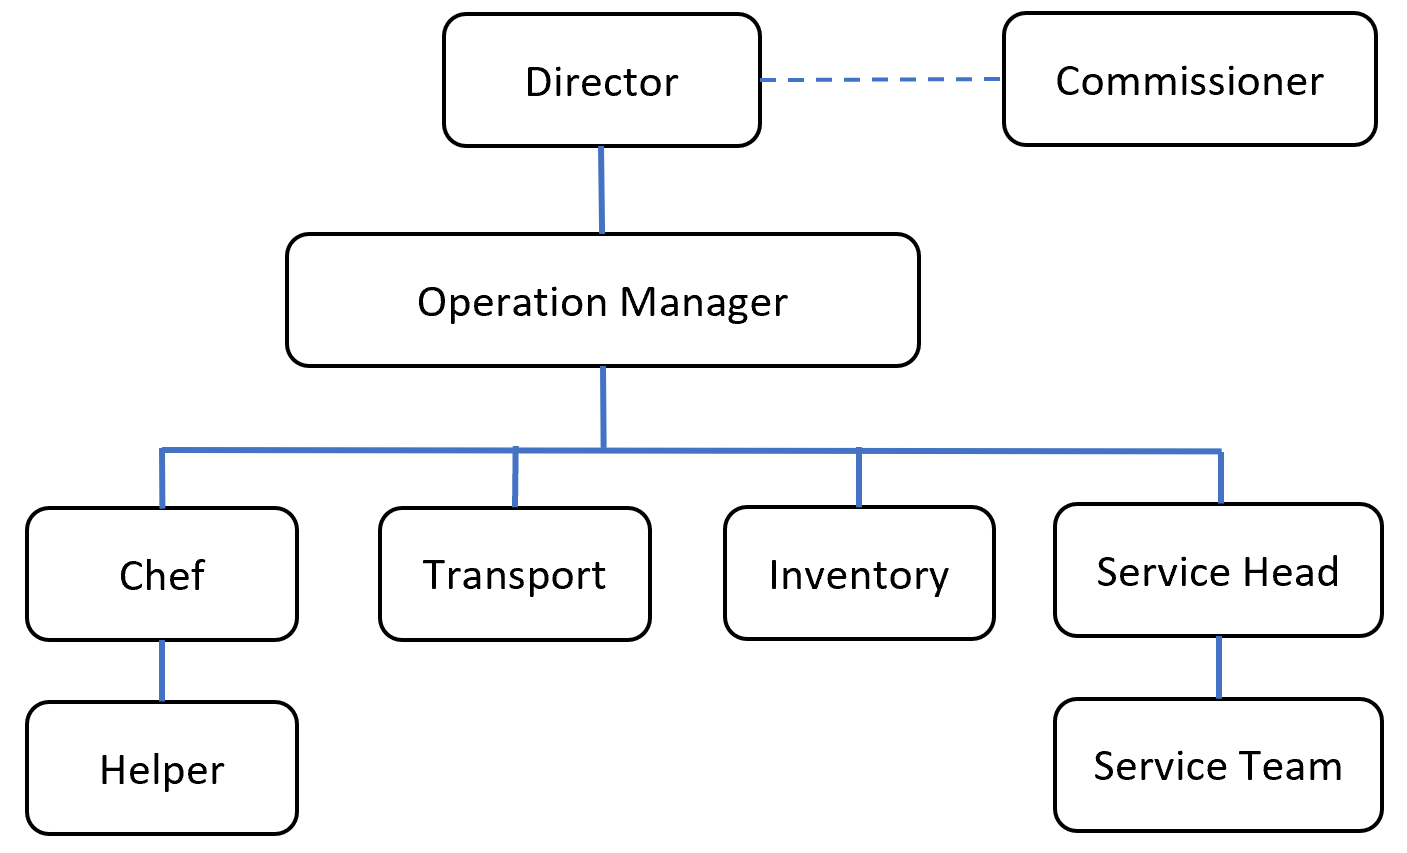
\includegraphics[width=10cm]{img/struktur-org.png}
    \caption{Struktur Perusahaan.}
    \label{gambar:struktur-org}
    \end{center}
\end{figure}

\subsection{Tugas dan Tanggung Jawab}
Struktur organisasi yang dimiliki oleh PT. BPS terbagi atas beberapa bagian yang memiliki 
fungsinya masing-masing. 
Berikut adalah penjelasan singkat tugas dan tanggung jawab dari masing-masing posisi divisi sebagai berikut:

\begin{enumerate}
    \item  \emph{Director}
        \begin{itemize}
        \item mengawasi dan mengarahkan jalannya perusahaan sesuai dengan visi dan misi.
        \item Memantau kerja dari operational manager.
        \end{itemize}
    \item \emph{Commissioner} 
        \begin{itemize}
        \item Mengawasi jalannya perusahaan.
        \item Memberikan arahan kepada director jika diperlukan.
        \end{itemize}
    \item \emph{Operational Manager}
        \begin{itemize}
        \item Bertanggung jawab untuk memenuhi kebutuhan dari pelanggan.
        \item Mengelola pemasukan dan pengeluaran perusahaan.
        \end{itemize}
    \item \emph{Chef dan Helper}
        \begin{itemize} 
        \item Bertanggung jawab memproduksi menu hidangan sesuai dengan standar yang ditetapkan perusahaan.
        \item Bertanggung jawab terhadap kepatuhan penggunaan standar resep.
        \item Bertanggung jawab terhadap hasil olahan menu.
        \item Membantu koki untuk mempersiapkan bahan dan peralatan.
        \end{itemize}
    \item \emph{Transport}
        \begin{itemize} 
        \item Mengantar makanan sampai ke tujuan.
        \item Memastikan kendaraan siap untuk beroperasi.
        \item Membuat laporan dan evaluasi terhadap aktivitas perjalanan.
        \item \emph{Inventory} 
        \item Memonitor dan mengelola proses pemenuhan order secara berkala.
        \item Bertanggung jawab dengan jumlah persediaan barang.
        \item Mengontrol masuk dan keluarnya barang dari gudang persediaan.
        \end{itemize}
    \item \emph{Service}
    \begin{itemize}
    \item Melayani pelanggan dengan ramah.
    \item Memberikan pelayanan dengan cepat.
    \end{itemize}
\end{enumerate}

\section{Produk Perusahaan}

\subsection{Katering Umum}

PT. BPS berpengalaman pada layanan katering umum seperti pada perayaan khitanan, 
arisan, ulang tahun, dan perayaan lainnya. PT. BPS siap menyajikan hidangan terbaik dan layanan yang memuaskan. 
Beragam pelanggan dengan berbagai perayaan kegiatan telah mempercayakan PT. BPS.

\subsection{katering Kantor}
Beberapa perusahaan mengutamakan efisiensi waktu pada saat jam istirahat. 
Waktu yang terbuang dan rasa lelah ketika harus pergi keluar kantor untuk makan 
siang bisa ditangani dengan berlangganan paket makan siang. Dengan latar belakang tersebut, 
PT. BPS menawarkan sebuah solusi kepada perusahaan dalam hal jasa katering dengan berbagai 
macam gaya makanan sesuai dengan selera pelanggan. 
PT. BPS siap melayani perusahaan dan menjadi mitra penyedia katering.

\subsection{Katering Industri/Pabrik}
Fenomena pada saat makan siang di kawasan industri, karyawan harus antri dan berdesakan sehingga 
tidak dapat menikmati menu makan siang. Hal ini tidak perlu terjadi apabila kebutuhan makan siang 
karyawan pabrik dipercayakan kepada pihak yang berpengalaman. PT. BPS siap memberikan solusi menu makan 
siang sesuai dengan kebutuhan pabrik dan perusahaan dengan karyawan dalam jumlah besar. 
Cara pengemasan pelayanan pada industri berbeda dari acara pribadi.  
Layanan catering yang diberikan kepada bisnis pelanggan dengan standar tinggi dan profesional. 
PT. BPS memelihara catatan layanan yang sangat baik, 
tim profesional dan terlatih untuk melayani semua jenis katering Industri.

\section{Daftar Pelanggan Industri}

Sejak tahun PT. BPS berbadan hukum, sebagian dari pelanggan industri besar adalah:
\begin{multicols}{2}
\begin{itemize}
\item PT. HM Sampoerna Tbk.
\item PT. Philip Morris Indonesia
\item PT. JTEKT Indonesia
\item PT. Piolax Indonesia
\item PT. Nici Indonesia
\item PT. Yangtze Optical Fibre Indonesia (PT. YOFI)
\item PT. Essence Indonesia (PT. IFF)
\item PT. Tsuruta Indonesia
\item PT. Furukawa Automotive Systems Indonesia (PT. FASI)
\item PT. Surya Rengo Containers (PT. SRC)
\item PT. Hiruta Kogyo Indonesia
\item PT. Marugo Rubber Indonesia
\end{itemize}
\end{multicols}

\clearpage
\mychapter{3}{BAB III \\ GAMBARAN UMUM PERUSAHAAN}



\subsection{Kedudukan dan Koordinasi}

Kedudukan penulis ditugaskan oleh perusahaan untuk menjadi web developer yang bertujuan 
untuk melakukan pembuatan \emph{website} profil perusahaan sebagai media atau sarana untuk marketing.

Dalam perusahaan ini, penulis memberikan didamping oleh komisaris (commissioner) 
yang bertindak sebagai business development yang bertujuan untuk memberikan ide, 
masukan dan selain itu memonitor pekerjaan dan arahan dari direktur dalam menjalankan perusahaan. 
Koordinasi dari pelaksanaan kerja magang ini adalah commissioner yang dan 
sekaligus menjadi pembimbing lapangan.

\subsection{Tugas yang dilakukan} 

Pembimbing lapangan menginginkan \emph{website} profil perusahaan dapat diakses dengan cepat atau responsive dengan 
uptime yang tinggi dan dapat muncul pada halaman utama search engine. 
Selain hal tersebut, pembimbing lapangan memberikan requirement agar update 
dari \emph{website} tersebut dapat di record dan sewaktu-waktu dapat di lakukan roll back action, 
atau pengembalian versi sebelumnya pada \emph{website}.

Untuk memenuhi kebutuhan tersebut, penulis mencoba untuk membandingkan beberapa 
framework sebelum mengimplementasikannya pada \emph{website}, 
framework yang dibandingkan seperti Gatsby dan Hugo. 
Penulis pada akhirnya memilih framework Hugo pada \emph{website} profil perusahaan agar 
\emph{website} menjadi lebih responsive, menggunakan GIT untuk record update pada \emph{website} atau 
versioning control dan setting up environment.~\cite{progit} 

\pagebreak

Pada pemilihan framework, poin-poin yang dibandingkan yaitu seperti stabilitas suatu 
\emph{website}, performa kecepatan \emph{website} dalam menyajikan konten, keamanan \emph{website}, 
kemudahan dalam memperbaiki dan memperbaharui \emph{website} dikemudian hari, 
minimalist looks pada \emph{website} dan kemudahan dalam pencarian \emph{website} pada search engine.

Pembimbing lapangan menginginkan \emph{website} profil perusahaan dapat diakses dengan 
cepat atau responsive dengan uptime yang tinggi dan dapat muncul pada halaman utama search engine. 
Selain hal tersebut, pembimbing lapangan juga menginginkan \emph{website} yang dapat 
dipercaya dengan keamanan yang cukup kuat.

Untuk memenuhi kebutuhan tersebut, penulis mencoba untuk membandingkan beberapa framework sebelum 
mengimplementasikan pada \emph{website}, framework yang dibandingkan seperti Gatsby dan Hugo. Kedua framework 
tersebut merupakan situs statis generator yang terkenal. Penulis pada akhirnya memilih framework 
Hugo untuk membuat suatu \emph{website} profil perusahaan.

Pada pemilihan framework, poin-poin yang dibandingkan yaitu seperti stabilitas suatu \emph{website}, 
performa kecepatan \emph{website} dalam menyajikan konten, keamanan \emph{website}, kemudahan dalam memperbaiki dan 
memperbaharui \emph{website} dikemudian hari, minimalist looks pada \emph{website} dan 
kemudahan dalam pencarian \emph{website} pada search engine.
    
Salah satu cara menilai stabilitas adalah dengan membandingkan masalah pada Hugo di GitHub 
dengan masalah Gatsby di GitHub. Gatsby memiliki lebih banyak fitur yang menarik tetapi memiliki 
lebih banyak bug pada saat pengembangan \emph{website}. Mungkin hal stabilitas tidak bukan merupakan kriteria 
yang cukup penting menurut beberapa orang. Tetapi untuk beberapa orang, stabilitas 
pada pengembangan suatu \emph{website}suatu hal yang penting karena waktu yang dihabiskan 
untuk berusaha menemukan bug itu,~\cite{ref:freecodecamp}
Hugo dapat membangun situs web tanpa alat tambahan dalam waktu kurang dari 100 ms. 
Gatsby mampu membangun situs web dalam waktu sekitar 15 detik, tetapi ini tidak termasuk banyak alat tambahan. 
Gatsby menggunakan JavaScript, dan aplikasi JavaScript terkenal karena membutuhkan banyak modul Node untuk dijalankan. 
Situs statis cenderung lebih aman, tetapi masih perlu menyebutkan bahwa lebih banyak dependensi 
menghasilkan lebih banyak kode yang mungkin tidak sepenuhnya dapat percaya.~\cite{ref:freecodecamp}

Pada pengembangan \emph{website}, spesifikasi dari operating system (OS) 
yang digunakan pada server adalah Debian 10 yang dikenal dengan debian buster. 
Selanjutnya penulis menggunakan metode virtualisasi level linux container dimana 
linux container tersebut mempunyai OS terpisah dari OS yang dipakai oleh server tetapi 
menggunakan kernel yang sama seperti pada tabel 3.1. OS yang digunakan pada linux container 
merupakan OS minimum untuk menjaga efisiensi dari performa. Jadi penulis memilih menggunakan  
Alpine dan Ubuntu base yang mempunyai spesifikasi apda tabel 3.2.~\cite{thedocker}


\begin{table}[!htb]
    \caption{Spesifikasi Kernel}
    \begin{center}
    \begin{tabular}{|l|l|}
    \hline
    Kernel & Linux 7b5e391f252d 4.19.0-6-cloud-amd64\\
    \hline
    \end{tabular}
    \end{center}
 \end{table}

\begin{table}[htbp]
    \caption{Spesifikasi Container}
    \begin{center}
    \begin{tabular}{|c|c|c|}
        \hline
        Container & OS & Version\\
        \hline
        Hugo-bps & Alpine Linux & v3.10.2\\
        \hline
        Jupyter-notebook & Ubuntu & v18.04.3\\
        \hline
    \end{tabular}
    \end{center}
    \end{table}


Testing dilakukan oleh pembimbing lapangan dan direktur dengan mengakses \emph{website} profil perusahaan 
dan memberikan feedback. Selain itu, menggunakan \emph{website} grader (\emph{website}.grader.com) dan 
sucuri (sitecheck.sucuri.net) untuk mengetahui standar nilai performa, search engine optimalization (SEO), 
keamanan, dan responsifitas.

Penilaian dibagi berdasarkan kriteria dari performa \emph{website} seberapa cepat \emph{website} diakses, 
berapa besar data halaman yang di muat dan permintaan halaman dari sisi browser ke sisi server.  
Kriteria yang menentukan SEO yaitu sitemap membantu untuk para websmaster 
yang mempermudah dalam pengenalan dalam \emph{website}, terdapat meta description yang memberikan 
penjelasan singkat dari isi dan halaman \emph{website}. 

Terdapat Secure Socket Layer (SSL) adalah lapisan 
keamanan untuk melindungi transaksi di \emph{website} dengan teknologi enkripsi dan memberikan kepercayaan 
pengunjung terhadap \emph{website} yang diaksesSemua requirement yang diminta hampir semuanya terpenuhi. 
Semua requirement yang diminta hampir semuanya terpenuhi. 
Dokumentasi dilakukan keseluruhan proses kerja magang dan penulisan 
laporan kerja magan selama proses pembuatan \emph{website} profil perusahaan.

\begin{figure}[htbp]
    \begin{center}
    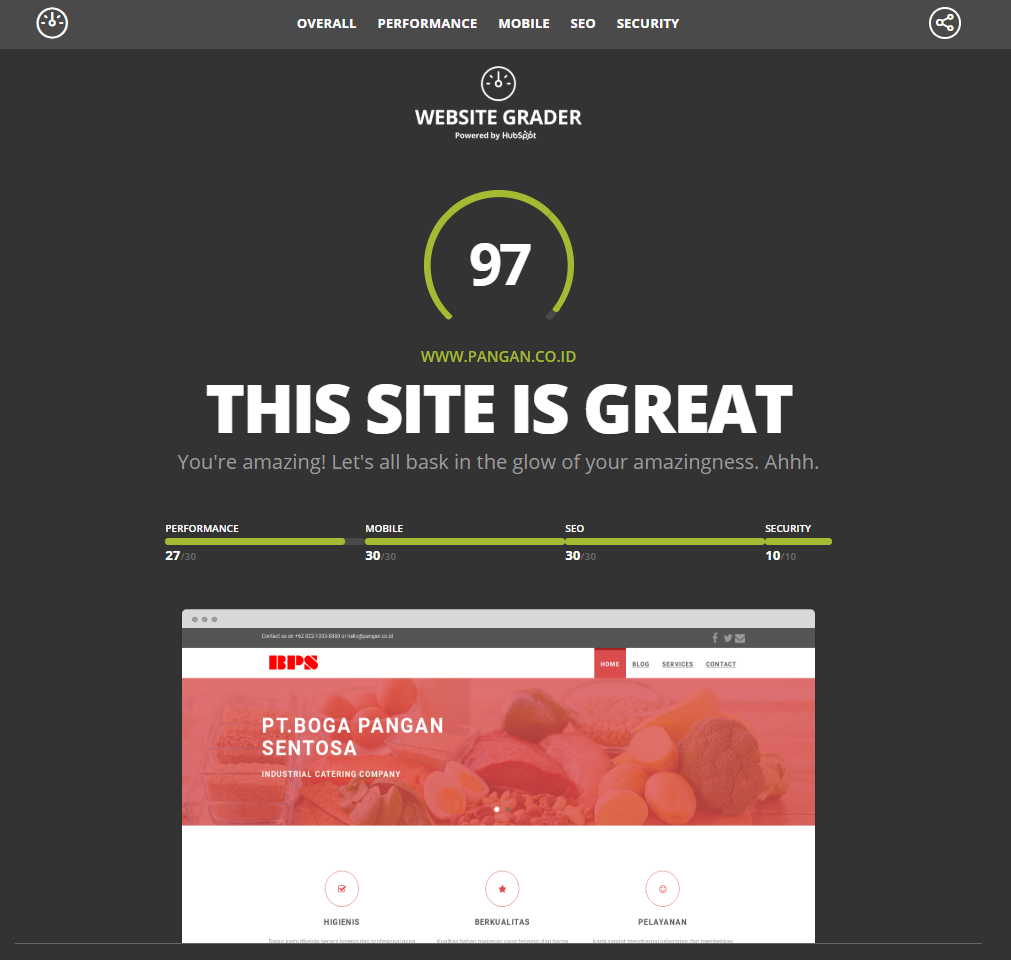
\includegraphics[width=10cm]{img/scr-website-grader.png}
    \caption{Standar nilai Performa \emph{website} pangan.co.id.}
    \label{gambar:scr-website-grader}
    \end{center}
\end{figure}

Dikarenakan penulis tidak ahli dalam bidang security maka penulis menggunakan 
online tools site checker security dan malware. Sucuri merupakan \emph{website} checker untuk 
mengetahui keamaan dan malware pada \emph{website} pangan.co.id. Hasil dari \emph{website} checker 
bahwa \emph{website} pangan.co.id tidak ditemukan malware, tidak adanya injected spam, 
tidak ada defacement, dan tidak ada internal error.didengan kata lain low security risk. 
Tidak adanya ancaman dari keamanan \emph{website}.

\begin{figure}[htbp]
    \begin{center}
    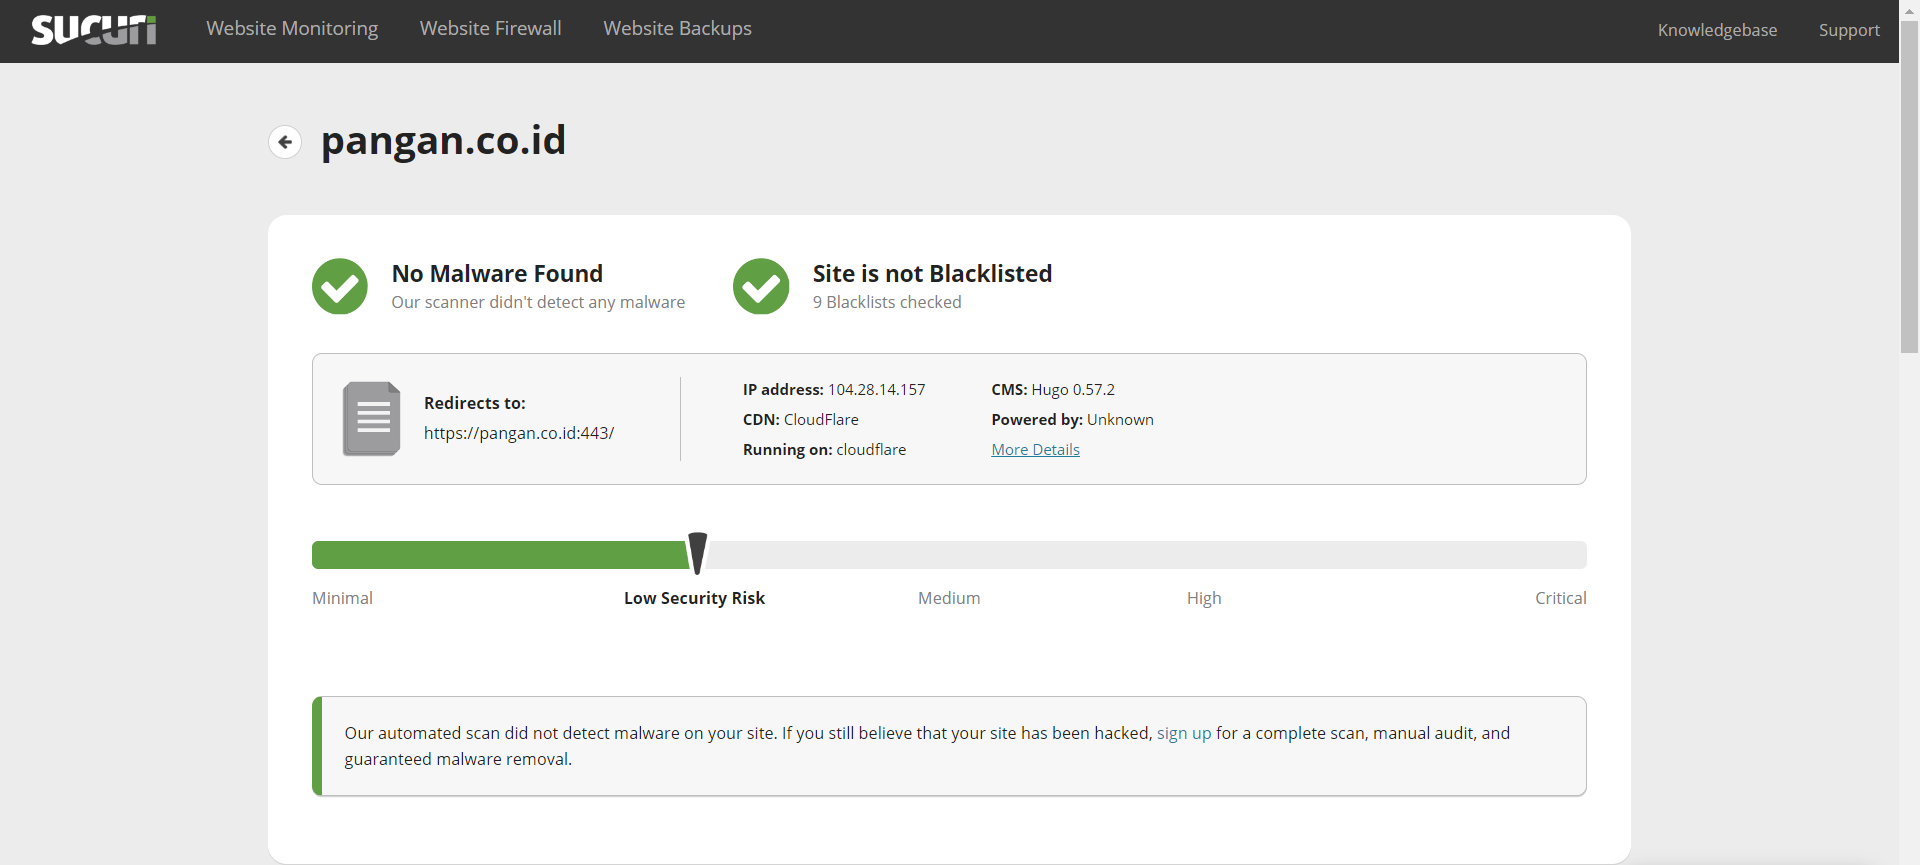
\includegraphics[width=10cm]{img/scr-suculi.png}
    \caption{Standar nilai keamanan dan malware checker}
    \label{gambar:scr-sucuri}
    \end{center}
\end{figure}

\pagebreak
Timeline kerja magang yang dilakukan penulis selama empat belas minggu serperti pada tabel 3.3

% Please add the following required packages to your document preamble:
% \usepackage{multirow}
\begin{table}[!htbp]
    \caption{Timeline Kerja Magang}
    \begin{tabular}{|l|l|l|l|l|l|l|l|l|l|l|l|l|l|l|l|}
    \hline
    \multicolumn{1}{|c|}{\multirow{2}{*}{No.}} & \multicolumn{1}{c|}{\multirow{2}{*}{Kegiatan}} & \multicolumn{14}{c|}{Minggu Ke}                            \\ \cline{3-16} 
    \multicolumn{1}{|c|}{}                     & \multicolumn{1}{c|}{}                          & 1 & 2 & 3 & 4 & 5 & 6 & 7 & 8 & 9 & 10 & 11 & 12 & 13 & 14 \\ \hline
    1                                          & Studi Literatur                                & x & x & x & x & x & x & x & x & x & x  & x  & x  & x  & x  \\ \hline
    2                                          & Requirement                                    & x & x &   &   &   &   & x &   &   &    &    &    &    &    \\ \hline
    3                                          & Instalasi dan setting-up                       &   & x & x &   &   &   &   &   &   &    &    &    &    &    \\ \hline
    4                                          & Implementasi                                   &   &   &   & x & x & x & x & x & x & x  &    &    &    &    \\ \hline
    5                                          & Testing                                        &   &   &   &   &   &   &   &   &   & x  & x  & x  & x  &    \\ \hline
    6                                          & Presentasi                                     &   &   & x &   &   & x &   &   & x &    &    & x  & x  &    \\ \hline
    7                                          & Dokumentasi                                    &   &   &   &   &   &   &   &   &   &    &    &    &    & x  \\ \hline
    \end{tabular}
    \end{table}


\subsection{Uraian Pelaksanaan Kerja Magang}

\subsubsection{Rancangan \emph{website}}
Gambaran sederhana yang dilakukan pengguna pada \emph{website} profil perusahaan dengan melihat halaman utama, 
blog, services dan contact us. \emph{website} profil perusahaan merupakan representasi 
perusahaan yang berisi informasi lengkap mengenai perusahaan dalam bentuk digital. 
Hal ini  memberi kesempatan bagi siapapun untuk mengakses dan menjadi nilai yang baik untuk masa depan perusahaan. 
Perancangan \emph{website} profil perusahaan akan dijelaskan lebih detail pada diagram arsitektur, 
menu hierarki diagram \emph{website} dan diagram use casee dan diagram arsitektur.

\subsubsection{Diagram Arsitektur}
Ruang lingkup dari \emph{website} profil perusahaan terdapat 3 linux container yaitu Hugo, 
Jupyter-notebook, dan traefik.  Traefik adalah proxy server dalam level micro-service 
untuk mengatur balance slot dan port forward. Ketiga container tersebut menggunakan kernel 
yang sama yaitu pada kernel Host OS. Traefik membuka akses port 80 (HTTP) dan 443 (HTTPS) ke 
jaringan agar dapat diakses oleh publik. Sedangkan Hugo dan jupyter memiliki internal network  
yang diatur oleh traefik 

Jupyter-notebook merupakan wadah untuk admin mengubah, menambah, menghapus konten. 
Memudahkan admin karena ‘wysiwyg’ what you see is what you get.\\

\begin{figure}[htbp]
    \begin{center}
    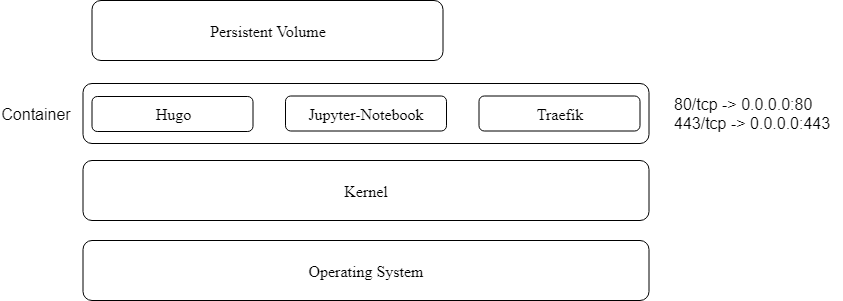
\includegraphics[width=15cm]{img/diag-arsitektur.png}
    \caption{Diagram Arsitektur}
    \label{gambar:diag-arsitektur}
    \end{center}
\end{figure}

\pagebreak
\subsubsection{Menu Hierarki Diagram \emph{website}}
\emph{website} profil perusahaan memiliki beberapa menu utama yang terdapat pada navigation bar. 
Menu utama berfungsi untuk memudahkan user untuk  berpindah halaman. 
Menu utama terbagi menjadi 4 yaitu Home, Blogs, Services dan Contact Us. 
Menu home memiliki konten nilai perusahaan, testimoni dari pelanggan, 
terdapat tombol untuk mengunduh company profile, recent post dari blog, dan client. 
Pada menu blogs, yang berisikan artikel-artikel. Menu Services berisikan uraian layanan yang 
ditawarkan perusahaan. 
Menu Contact Us berisikan informasi kontak perusahaan pada halaman ini pengunjung dapat mengisi 
form atau menghubungi nomor yang tertera pada halaman tersebut.

\begin{figure}[htbp]
    \begin{center}
    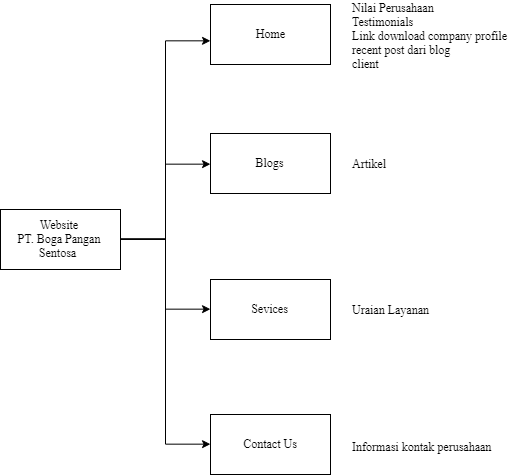
\includegraphics[width=12cm]{img/diag-menu.png}
    \caption{Hirarki Menu Diagram \emph{website}}
    \label{gambar:diag-menu}
    \end{center}
\end{figure}

\pagebreak
\subsubsection{Diagram Use Case}

Diagram use case merupakan pemodelan untuk menggambarkan kelakuan sistem yang akan dibuat. 
Diagram use case mendeskripsikan sebuah interaksi antara satu atau lebih aktor dengan sitem yang akan dibuat[4]. 
Diagram ini digunakan untuk mengetahui fungsi apa saja yang ada di dalam suatu sistem dan siapa saja yang berhak 
menggunakan fungsi tersebut[4]. Pada diagram Use Case, terdapat 2 aktor yaitu User dan Admin. User pengguna 
dapatmemiliki akses Read Only (RO) seperti:  melihat informasi mengenai PT. BPS, melihat layanan PT.BPS, melihat 
artikel blog, melihat informasi contact service. Sedangkan Admin memiliki kewenangan untuk dapat melakukan Create, 
Read, Update dan Detete (CRUD) terhadap suatu konten. 

\begin{figure}[htbp]
    \begin{center}
    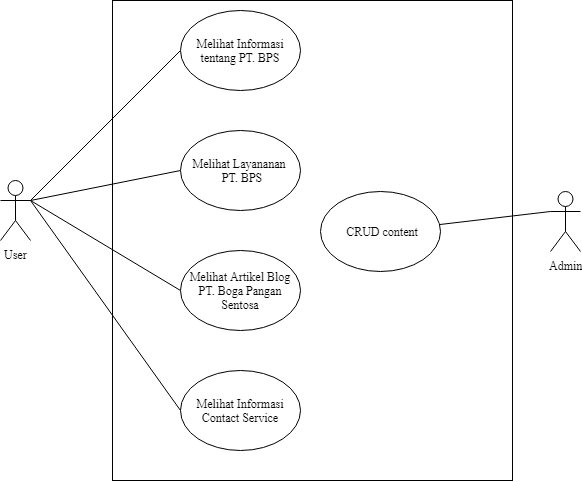
\includegraphics[width=12cm]{img/diag-usecase.png}
    \caption{Diagram Use Case}
    \label{gambar:diag-usecase}
    \end{center}
\end{figure}

\subsubsection{Implementasi \emph{website}}
Admin dapat mengunakan alamat situs note.pangan.co.id 
dimana \emph{jupyter notebook} di \emph{install}. yang berguna 
untuk membuang atau menambahkan konten.  
Admin menuju ke folder content > blogs untuk menambahkan artikel pada halaman blogs. 
Admin harus mengetahui bagaimana cara menulis artikel pada \emph{markdown} (md). 
Penulis memberikan panduan cara menulis artikel dengan format (md). 

\begin{figure}[htbp]
    \begin{center}
    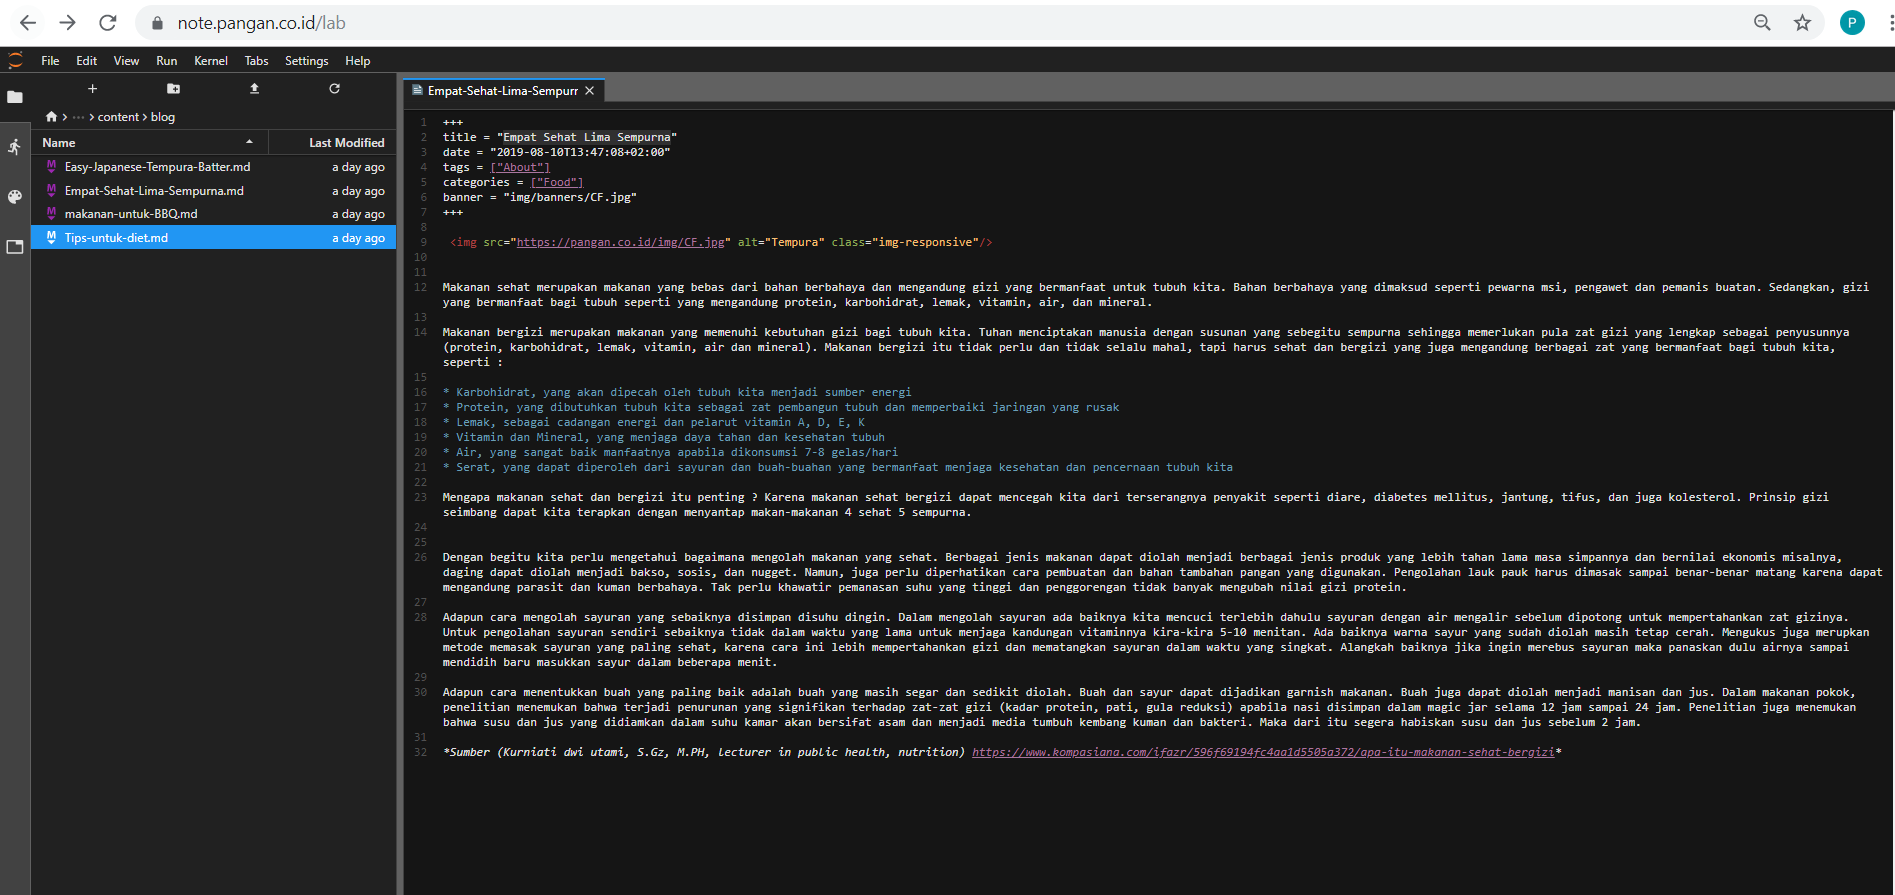
\includegraphics[width=12cm]{img/scr-adm-1.png}
    \caption{Jupyter Notebook section blog}
    \label{gambar:scr-adm-1}
    \end{center}
\end{figure}


Berikut Tampilan folder listing yang dapat diakses oleh admin. Untuk mengubah suatu konten, 
Admin harus mengakses folder “content” lalu terdapat folder “blog”.

\begin{figure}[htbp]
    \begin{center}
    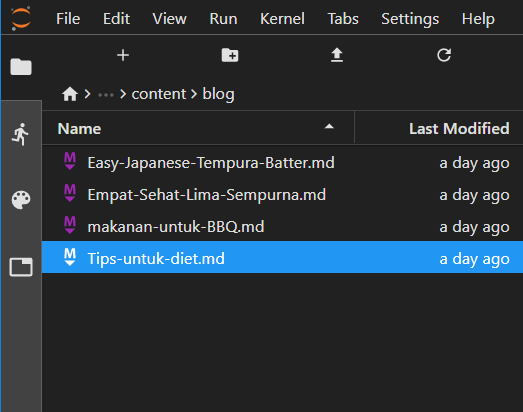
\includegraphics[width=7cm]{img/scr-adm-2.png}
    \caption{Folder Listing}
    \label{gambar:scr-adm-2}
    \end{center}
\end{figure}


\begin{figure}[htbp]
    \begin{center}
    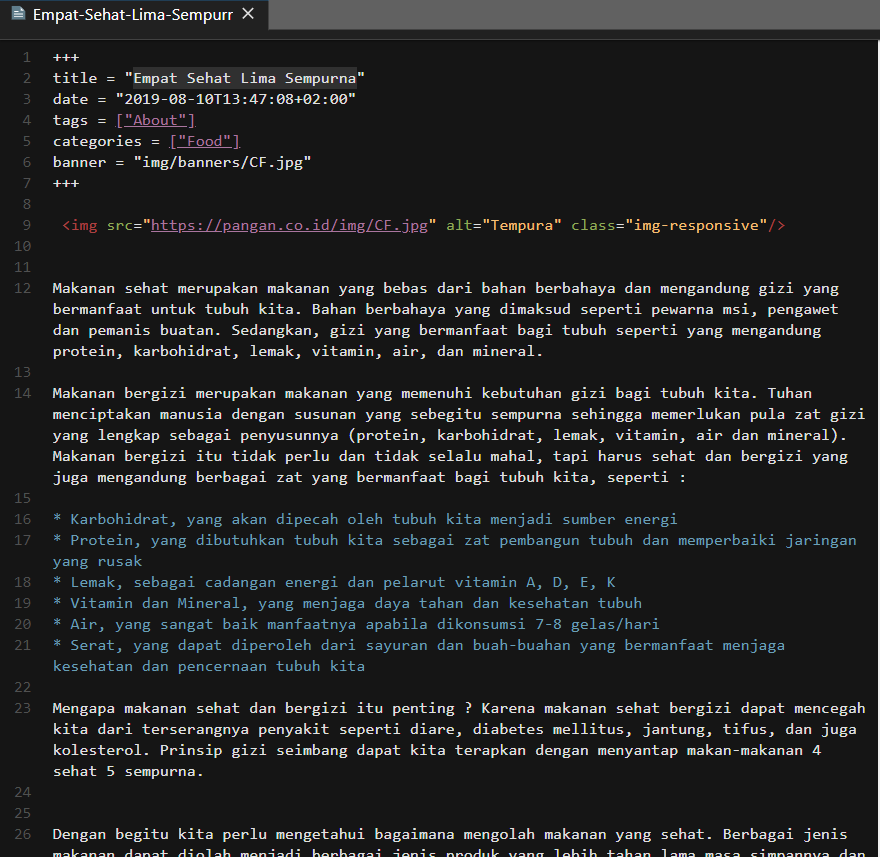
\includegraphics[width=8cm]{img/scr-adm-3.png}
    \caption{Tampilan edit dengan format markdown}
    \label{gambar:scr-adm-3}
    \end{center}
\end{figure}

Selain menambah artikel pada blog admin dapat mengubah lainnya seperti uraian pada service, 
kontak perusahaan, atau menambah testimonial dari pelanggan.

\begin{figure}[htbp]
    \begin{center}
    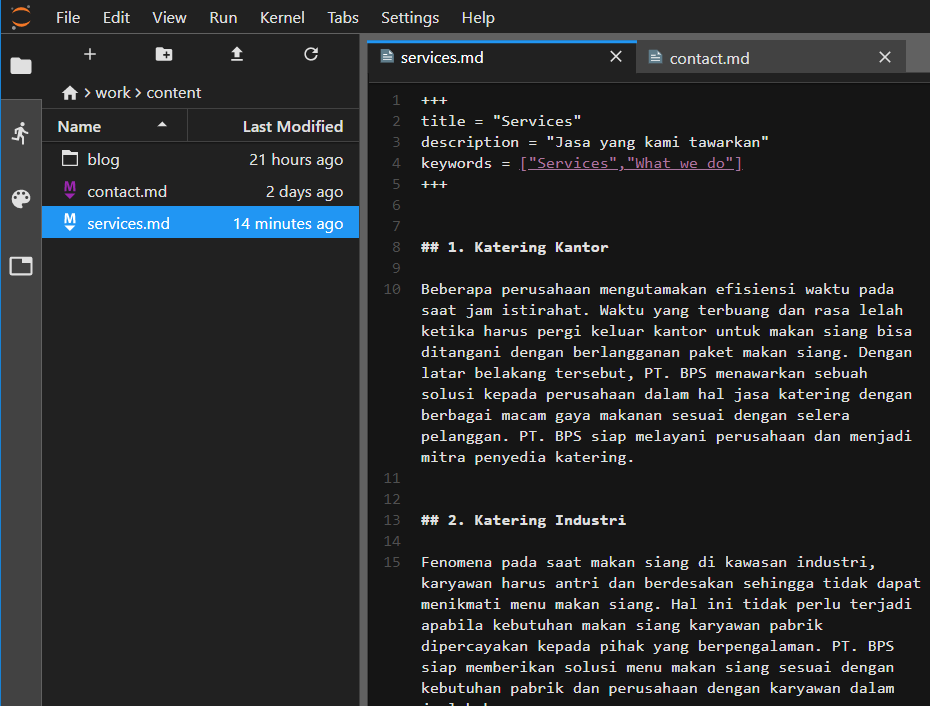
\includegraphics[width=8cm]{img/scr-adm-4.png}
    \caption{Tampilan edit services.md dan contact.md}
    \label{gambar:scr-adm-4}
    \end{center}
\end{figure}


Pada \emph{website} profil perusahaan, halaman utama terdiri dari carousel, nilai perusahaan, 
terstimonial, banner, recent post, client, footer. Bagian navigation bar berisi Home, 
Blog, Service dan Contact. Testimoni dari pelanggan yang sudah berlangganan dengan 
PT. BPS. Banner yang tertera pada halaman utama. Jika pengguna ingin mengetahui 
PT. BPS lebih lanjut, pengguna dapat menekan tombol 
“Check other homepages” yang akan mengunduh company profile. 


% Tampilan Webiste
%
%

\begin{figure}[htbp]
    \begin{center}
    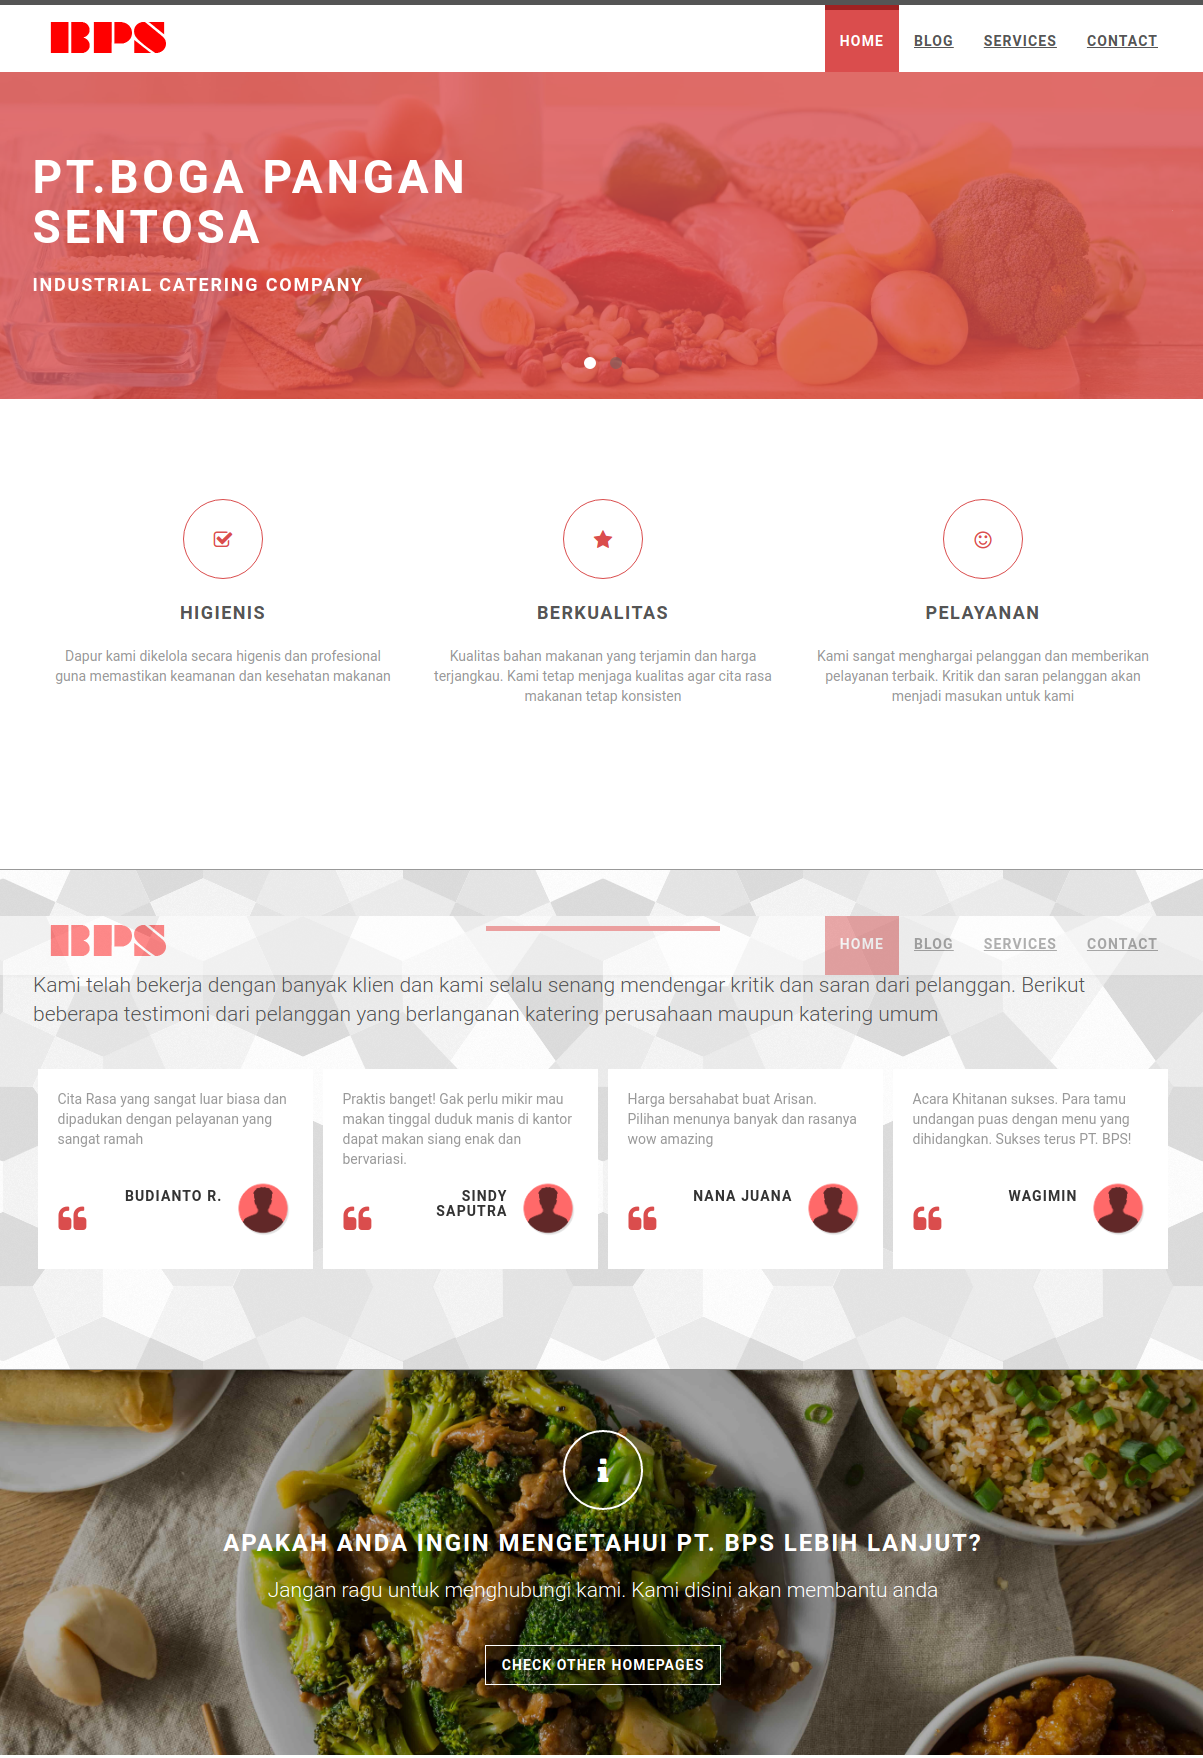
\includegraphics[width=7cm]{img/scr-website-1.png}
    \caption{Halaman Utama}
    \label{gambar:scr-website-1}
    \end{center}
\end{figure}

Pada recent post menampilkan empat artikel terakhir yang ditambahkan oleh admin. 
User dapat mengarahkan kursor ke gambar atau tombol continue reading,  
akan mebuka halaman blog. Bagian Our Clients terdapat beberapa logo perusahaan yang menjadi 
pelanggan dan merasakan hidangan dan pelyanan yang  diberika oleh 
PT. BPS. Footer terdapat pada setiap halaman, 
Footer terbagi menjadi beberapa bagian yang menampilkan about us secara singkat, 
recent posts, contact, dan copyright.

% Blog
%
%

Halaman ini memuat artikel yang berkategori tips, resep, dan makanan. 
Blogs dibuat dengan harapan selain melihat company profile dari BPS, 
juga dapat melihat artikel-artikel. Side menu yang berisikan search, 
categories, dan tags yang memudahkan user dalam pencaharian artikel yang ingin dibaca.

\begin{figure}[htbp]
    \begin{center}
    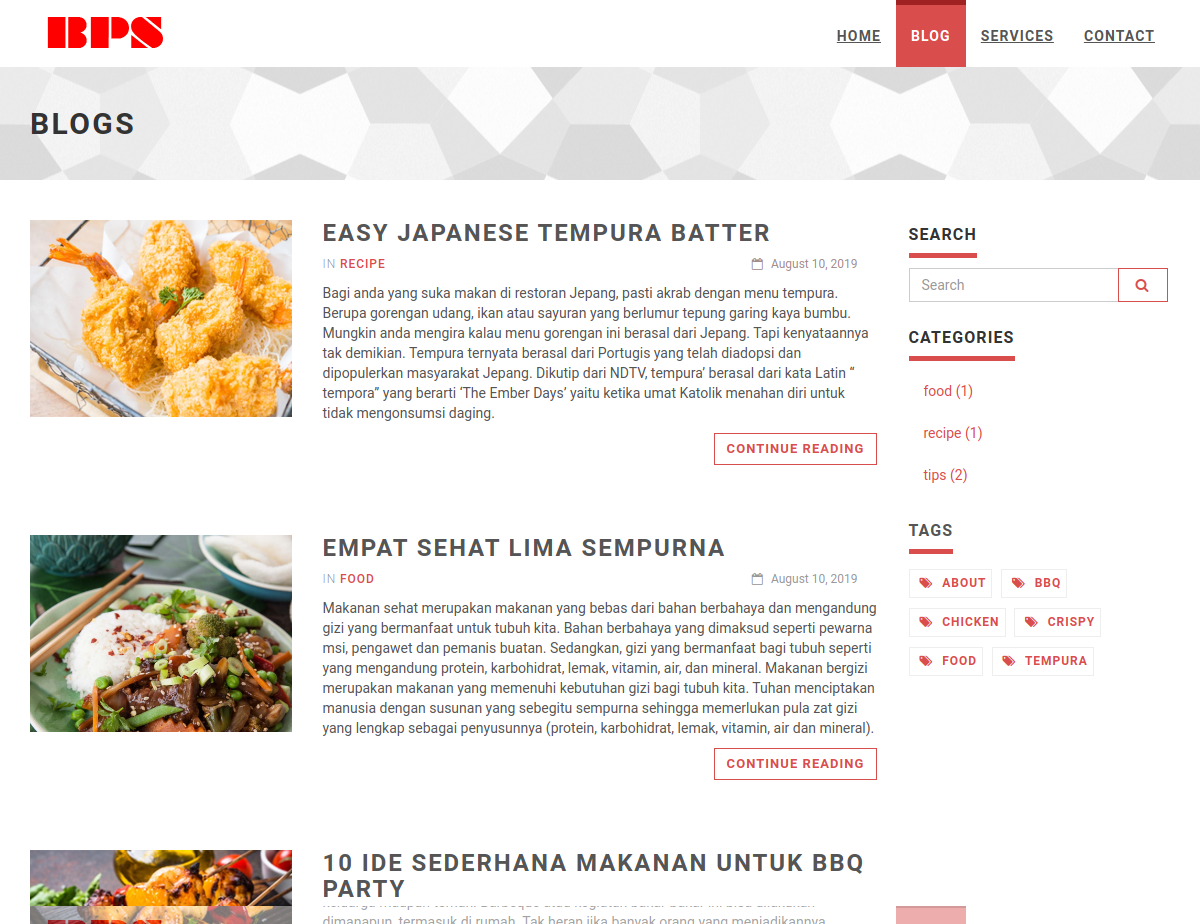
\includegraphics[width=8cm]{img/scr-website-blog.png}
    \caption{Halaman Blog}
    \label{gambar:scr-website-blog}
    \end{center}
\end{figure}


Halaman services yang berisikan uraian pelayanan yang ditawarkan perusahaan 
PT. BPS menawarkan katering kantor, karting industry dan katering umum. Calon 
pelanggan dapat memilih sesuai dengan kebutuhan dari perusahaan. 
Jika calon pelanggan ingin mengetahui lebih lanjut dapat menjutu navigation bar dan menekan tombol contact

\begin{figure}[htbp]
    \begin{center}
    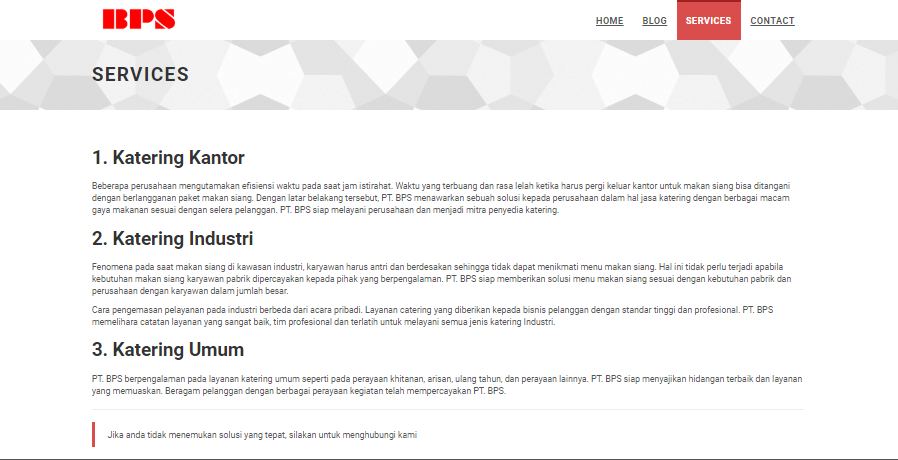
\includegraphics[width=8cm]{img/scr-website-service.png}
    \caption{Halaman Service}
    \label{gambar:scr-website-service}
    \end{center}
\end{figure}

Halaman contact terdiri dari contact form, telepon, dan alamat perusahaan. 
Calon pelanggan yang tertarik dengan layanan yang diberikan oleh perusahaan dapat langsung mengisi 
contact form dan akan langsung terkirim \\ke hello@pangan.co.id.  
Calon pelanggan mengunjungi alamat perusahaan atau menelfon di nomor layanan yang tertera.

\begin{figure}[htbp]
    \begin{center}
    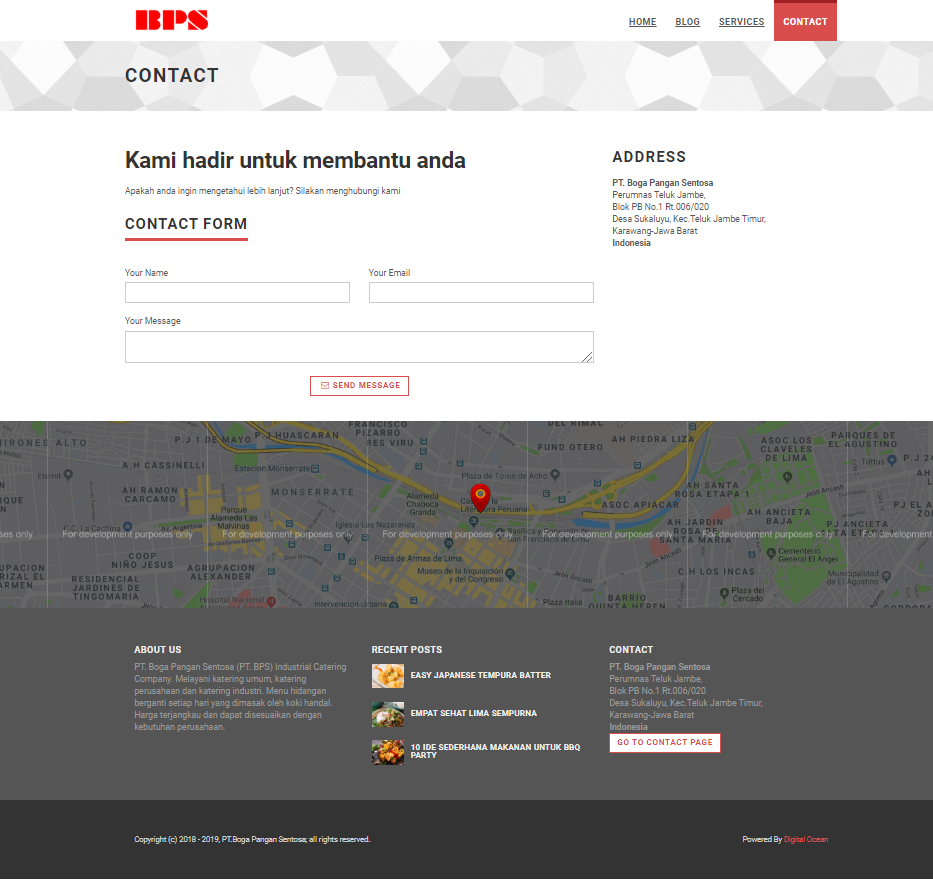
\includegraphics[width=5cm]{img/scr-website-contact.png}
    \caption{Halaman kontak}
    \label{gambar:scr-website-contact}
    \end{center}
\end{figure}

\subsection{Kendala yang ditemukan}

Pada proses pembuatan \emph{website} profil perusahaan terdapat kendala yang ditemukan 
seperti sulitnya mengisi konten \emph{website} dikarenakan minimnya informasi dan 
dokumentasi yang layak dari perusahaan. Selain itu kendala yang lain yaitu user acceptance. 
User Acceptance adalah tahap akhir pada testing yang 
dijalankan untuk mengetahui apakah masih terdapat kecacatan pada \emph{website} yang dikembangkan.

\subsection{Solusi atas kendala yang ditemukan}
Solusi untuk menyelesaikan kendala 3.4 yaitu dengan \emph{gathering} data perusahaan dan 
menampilkam beberapa dokumentasi yang layak. 
Untuk menyelesaikan masalah \emph{user acceptance} yaitu melakukan \emph{survey} dengan melakukan wawancara. 

\clearpage
\begin{center}
    \textbf{BAB IV \\ SIMPULAN DAN SARAN}
    \addcontentsline{toc}{section}{BAB IV SIMPULAN DAN SARAN}
\end{center}
\setcounter{section}{4}
\setcounter{subsection}{0}

\subsection{Simpulan}

Pelaksanaan kerja magang telah selesai dilaksanakan. Website profil perusahaan 
PT. BPS digunakan sebagai marketing untuk meningkatkan sales. Website profil 
perusahaan dibuat menggunakan framework Hugo memenuhi requirement dari segi performa kecepatan, 
SEO, responsif, dan keamanan. Pengalaman kerja yang didapatkan sangat berarti karena pada 
PT. BPS penulis diberikan ruang berkreasi untuk memilih 
framework dan mengimplementasikan ke pada website profil perusahaan. Selama kerja magang, 
penulis juga diajarkan untuk mempertahankan argumentasi, berkomunikasi dengan tegas dan efektif.

\subsection{Saran}
Hasil kerja magang telah dilaksanakan dan saran untuk pengembangan website kedepannya sebagai berikut:
\begin{enumerate}[label=(\alph*)]
\item Membuat halaman portfolio dengan menambahkan foto gallery.
\item Pada website harus ditampilkan perencanaan menu untuk satu bulan sehingga para 
pelanggan kantor atau umum dapat memesan menu yang sesuai dengan menu yang ada dalam daftar.
\item Dapat menampilkan berapa nilai kepuasan pelanggan terhadap pelayanan PT. BPS. 
Nilai tersebut diambil dari hasil kuesioner.
\item Menambahkan pesanan makanan dalam bentuk paket pernikahan, sarapan pagi, 
pesta ulang tahun, dll. Sehingga dapat memberikan ide bagi pelanggan untuk memesan menu yang sesuai.
\end{enumerate}

\clearpage
\begin{center}
    \textbf{Daftar Pustaka}
    \addcontentsline{toc}{section}{Daftar Pustaka}
\end{center}

\noindent [1] DZone, 2019. Static Site Generator Overview: Gatsby vs. Hugo vs. Jekyll. [online]\\
 Tersedia di : https://dzone.com/articles/static-site-generators-overview-gatsby-vs-hugo-vs [Diakses Senin 24 Juni 2019]\\
\noindent [2] freecodecamp, 2018. Gatsby vs Hugo, a detailed comparison.[online] 
\\Tersedia di: https://www.freecodecamp.org/news/gatsby-vs-hugo-a-detailed-comparison-e78d94f640fc/  [Diakses Senin 24 Juni 2019 ]\\
\noindent [3] Dewaweb. Apa itu SSL (secure socker layer)?.[online] 
\\Tersedia di:  https://www.dewaweb.com/index.php?rp=/knowledgebase/86/Apa-itu-SSL-Secure-Socket-Layer.html [Diakses Rabu, 26 Agustus 2019]\\
\noindent [4] PcControl, Pengetahuan dasar diagram use case. [online] 
\\Tersedia di : https://pccontrol.wordpress.com/2012/08/23/pengetahuan-dasardiagram-use-case/ [Diakses Senin 16 September 2019]\\


%\section{Daftar Pusataka}
%\clearpage
%\begin{flushleft}

%\bibliographystyle{unsrt}
%\bibliography{pustaka}
  
%\end{flushleft}

%\printbibliography[title={DAFTAR PUSTAKA}]

\end{document}